\documentclass[12pt]{report}
% \usepackage{minted}
\usepackage{xcolor}
\definecolor{light-gray}{rgb}{0.9,0.9,0.9}
% \usepackage{emptypage}
\usepackage[T1]{fontenc}
\usepackage{textcomp}
\usepackage[utf8]{inputenc}
% \usepackage[italian]{babel}
\usepackage{graphicx}
\graphicspath{ {Images/} }
\usepackage{caption}
\usepackage{subcaption}
\usepackage{enumerate}
\usepackage{array}
\usepackage{tabularx}
\usepackage{float}
\usepackage[a4paper,width=150mm,top=30mm,bottom=30mm,left=30mm,right=30mm,bindingoffset=6mm]{geometry}
\usepackage{fancyhdr}
\linespread{1.3}\selectfont

\usepackage{titlesec}
\titleformat{\chapter}{}{}{0em}{\bf\LARGE}

\usepackage{hyperref}
\hypersetup{
    colorlinks,
    citecolor=black,
    filecolor=black,
    linkcolor=black,
    urlcolor=black
}


\begin{document}
  %TODO: run a spellcheck
  %TODO: check id SafeStreets is well written in all files (i.e. missing final s)
  % TODO: Fill title page
  \begin{titlepage}
    \begin{figure}[t]
        \centering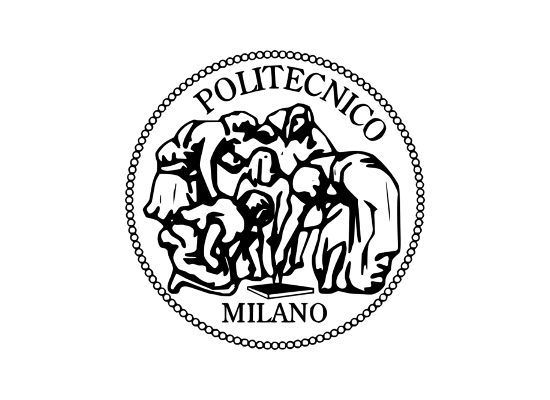
\includegraphics[width=0.5\textwidth]{Images/logo_polimi}
    \end{figure}
    \begin{center}
        \textsc{ \LARGE{Politecnico di Milano \\}}
      \textsc{ \LARGE{Dipartimento di Energia, Informazione e Bioingegneria\\ }}
      \textnormal{ \LARGE{Computer science and engineering \\ Software engineering 2\\}}
      \vspace{30mm}
      \fontsize{10mm}{7mm}\selectfont 
        \textup{SafeStreets - DD}\\
    \end{center}
    
    \vspace{25mm}
    
    \begin{minipage}[t]{0.47\textwidth}
      \textnormal{\large{\bf Professor:\\}}
      {\large Prof. Elisabetta Di Nitto}
    \end{minipage}\hfill\begin{minipage}[t]{0.47\textwidth}\raggedleft
      \textnormal{\large{\bf Candidates:\\}}
      {\large Nicolò Albergoni - 939589\\}
      {\large Luca Loria - 944679}
    \end{minipage}
    
    \vspace{20mm}
    
    \centering{\large{Academic Year 2019/2020 \\ Milano - 09/12/2019 }}
    
  \end{titlepage}
  
  
  \tableofcontents
   
  \chapter{Introduction}
  \section{Purpose}
  The purpose of this Requirement Analysis and Specification Document (RASD)
is to provide a detailed description about SafeStreets.
In particular, this document is focused on important aspects that are
useful during the design of the software architecture like: scope, functional and
non-functional requirements, use cases and scenarios, constraints and assumption, UML diagrams, limitation and interfaces with other software.
Overall the document is a useful guide for the developers that will have to follow
and implement all the necessary requirements; nevertheless it is also a document
that can be given to potential customers to get them an idea of what the software
will be like.\newline
The software features have been identified in the following list of goals.

\subsection{Goals}
\begin{itemize}
  \item {[G1]}: Allow a person to become a registered User after submitting his credentials for the registration to the service
  \item {[G2]}: Allow the user to send a violation report consisting in a picture and some metadata
    \begin{itemize}
      \item {[G2.1]}: Allow the user to send along with the picture the plate number
    \end{itemize}
  \item {[G3]}: Allow the user to watch the history of his reports and their status
  \item {[G4]}: Allow the user to watch on a map areas and streets with an high frequency of violations
  \begin{itemize}
    \item {[G4.1]}: The user gets the latest violations near its current location 
    \item {[G4.2]}: The user gets the latest violations near the location that he specifies
  \end{itemize} 
  \item {[G.5]}: Allow the local system administrator of the police station to create accounts for the police technician by giving him an administrator account
  \item {[G.6]}: Allow the authorities to visualize the reports submitted by the users
  \item {[G.7]}: Allow the authorities to mine the data to make analisys and retrieve statistics
  \item {[G.8]}: If the municipality offers a service that provides data about accidents then the system must be able to cross this data with its own data in order to identify possible unsafe areas
  \begin{itemize}
    \item {[G.8.1]}: In this case the system must be able to suggest possible interventions
    \item {[G.8.2]}: The users must be able  watch this unsafe areas
    \item {[G.8.3]}: The authorities must be able to consult the crossed data
  \end{itemize} 
\end{itemize}


  \section{Scope}
  % TODO: check the scope
Here is a brief review of what has already been said into the RASD document about the SafeStreet scope and functionalities.
\newline
SafeStreets is a new service that aims, via the help of citizens, to improve the safety of the streets. Users will have the possibility to send reports of illegal behaviour related to street parking to authorities, just by opening the safe SafeStreets mobile application and take a picture of the violation. Moreover they can also consult the history of their reports and a map that will highlight the most dangerous streets nearby. SafeStreets also offers a way for the authorities to manage the reports and perform analysis on the data. A Web interface will be developed in order to address this purpose. In order to guarantee and efficient use of the application by authorities, the system interacts with an external plate recognition service that will extract the car plate number from the report image. In this way when authorities need to check on a report they immediately find the car plate number of the vehicle that committed the violation. SafeStreets also implements a functionality that performs the interaction with a municipality service that offers data regarding car accidents, if the particular municipality offers one. SafeStreets can cross this information with its owns, in order to get a better idea of the potentially unsafe areas and therefore suggest some possible interventions.
As for the performances, the service will have to be scalable,
fast and it must be able to cover a great number of users. While for the applications they must be lightweight and must run of most of the devices available on the market.

  \section{Definitions, acronyms and abbreviations}
  \subsection{Definitions}
\begin{itemize}
  \item \textit{Most Dangerous Streets}: Streets with the highest frequency of violation reports.
\end{itemize}

\subsection{Acronyms}
\begin{itemize}
  \item EU: European Union;
  \item CET: Central European Timezone;
  \item API: Application Programming Interface;
  \item HTTP: Hyper Text Transfer Protocol;
  \item GPS: Global Positioning System;
  \item GDPR: General Data Protection Regulation;
  \item REST: Representational State Transfer.
  \item URL: Uniform resource locator
  \item URI: Uniform resource indicator
  \item DB: Database
  \item DBMS: Database management system
  \item RDBMS: Relational database management system
  \item SQL: Structured query language
  \item NoSQL: Not only SQL
\end{itemize}

\subsection{Abbreviations}
\begin{itemize}
  \item {[Gn]}: n-th goal;
  \item {[Dn]}: n-th domain assumption;
  \item {[Rn]}: n-th functional requirements;
  \item MDS: Most Dangerous Street;
  \item LSA: Local System Administrator;
  \item PT: Police Technician.
\end{itemize}

  \section{Revision History}
  \begin{itemize}
    \item Version 1:
        \begin{itemize}
            \item 1.0: First release.
            \item 1.1: Minor fixes to sequence diagrams
        \end{itemize}
\end{itemize}

  \section{Reference Documents}
  \begin{itemize}
    \item LateX Workshop extension for Visual Studio Code: \newline\href{https://github.com/James-Yu/LaTeX-Workshop/}{https://github.com/James-Yu/LaTeX-Workshop/}
    \item LateX compiler: \newline\href{https://www.latex-project.org/}{https://www.latex-project.org/}
    \item StarUML for UML diagrams:\newline\href{http://staruml.io/}{http://staruml.io/}
    \item DrawIO for some UML diagrams\newline\href{http://draw.io}{http://draw.io}
    \item MVC design pattern wikipedia: \newline\href{https://en.wikipedia.org/wiki/Model-view-controller}{https://en.wikipedia.org/wiki/Model-view-controller}
    \item Multitier architecture wikipedia: \newline\href{https://en.wikipedia.org/wiki/Multitier_architecture}{wikipedia}
    \item Relational database advantages: \newline\href{https://searchdatamanagement.techtarget.com/definition/relational-database}{https://searchdatamanagement.techtarget.com/definition/relational-database}
\end{itemize}
  \section{Document Structure}
  % TODO: check if this list is still right
\begin{enumerate}
  \item In the first part a general introduction of the Design Document is given. The purpose part exposes the substantial differences with the RASD document;
  \item The second section it's the core of the DD: it firstly provides an high level overview of the system followed by  a description of various aspects of the architecture from different points of view such as: component, deployment and runtime view. It is also present a general explanation of the architectural patterns and styles adopted in the development process. Most of the parts of this section are enriched with UML diagrams to ensure a better understanding of the concepts;
  \item This part specifies the user interface design of the mobile application and the web interface. Since the mockups of both applications were already provided in the RASD document, here some UX diagrams are proposed to better describe the navigation and functioning of the applications;
  \item Part four exposes the requirements traceability matrix which maps the requirements stated in the RASD document with the corresponding design component;
  \item Chapter five provides the proposals for the implementation, integration and testing plans. This plans are created by taking into account, for each functionality, the importance for the customer and the difficulty of implementation/testing;
  \item The last part states the hours of work division and the tools used to create  all the part of this DD document.
\end{enumerate}

  
  \chapter{Architectural Design}
  \section{Overview: High-level components and their interaction}
  In this	section an analysis of some critical aspects of the system is provided exploiting Alloy.	
The	focus is on	some static	constraints, in	particular:	
\begin{itemize}
    \item Uniqueness of usernames and every other univoque parameter of the system, such as plates, violationIds and so on;
    \item Users can only mine information concerning MDS and not Plates. Also they cannot explicitly query reports that has been performed by other users;
    \item LSAs can deal only with violation occurred in their competence area and thus scheduling such violations to the technician that they manage;
    \item SuggestedIntervention can be generated only if at least one violation occurred in the same location of the suggestion.
\end{itemize}
Other constraints are specified for keeping a steady structure of the alloy model, in order to avoid dangling entities and preserving foreign constraints.\newline
Four different worlds have been generated in order to verify the correctness of the constraints.

  \section{Component view}
  The \ref{fig:component_diagram} represents the Safestreets component diagram. Each of the components are wrapped inside a specific box that indicates the subsystem in which they belong to.
\newline Subsystems are groups of components which perform similar operations: this boxing technique is a multilayer logical division that can be useful in order to categorize the components and the whole system at different layers of abstraction.
\newline For the sake of simplicity, the component diagram pictures the application layer (backend) of the system and not the mobile and web app structures. The business logic and core functions are fully contained in the application layer and therefore only that relevant part of the Safestreets system has been characterized.
\begin{figure}[H]
    \centering
    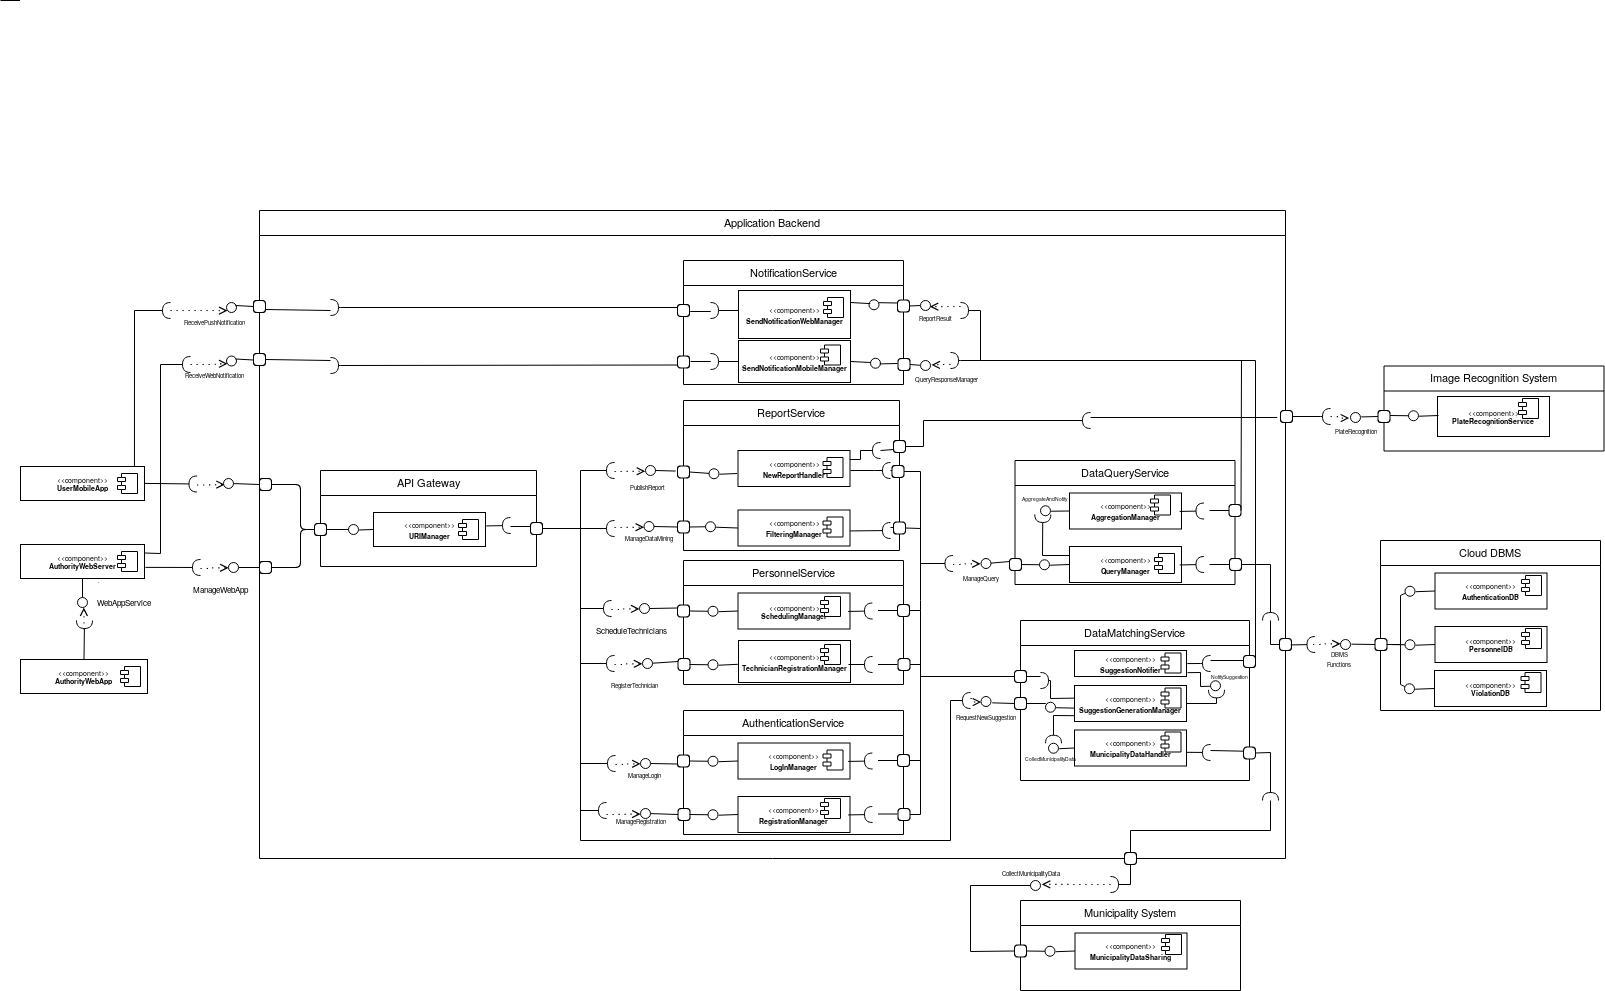
\includegraphics[width=1.1\textwidth]{UML_diagrams/component_uml_safestreets}
    \caption{Component UML diagram}
    \label{fig:component_diagram}
\end{figure}
Here it is a detailed explanation for each of the components shown in the component diagram:
\begin{itemize}
    \item 
    \item 
    \item 
    \item 
    \item 
    \item 
    \item 
    \item 
    \item 
    \item 
    \item 
    \item 
    \item 
    \item 
    \item 
    \item 
    \item 
    \item 
    \item 
    \item 
    \item 
    \item 
    \item 
\end{itemize}
  \section{Deployment view}
  The following image represents the deployment diagram of the SafeStreets architecture. It shows the logical division of the software architecture as well as the distribution of the software components to their target nodes, on which they will be deployed.

\begin{figure}[H]
  \centering
  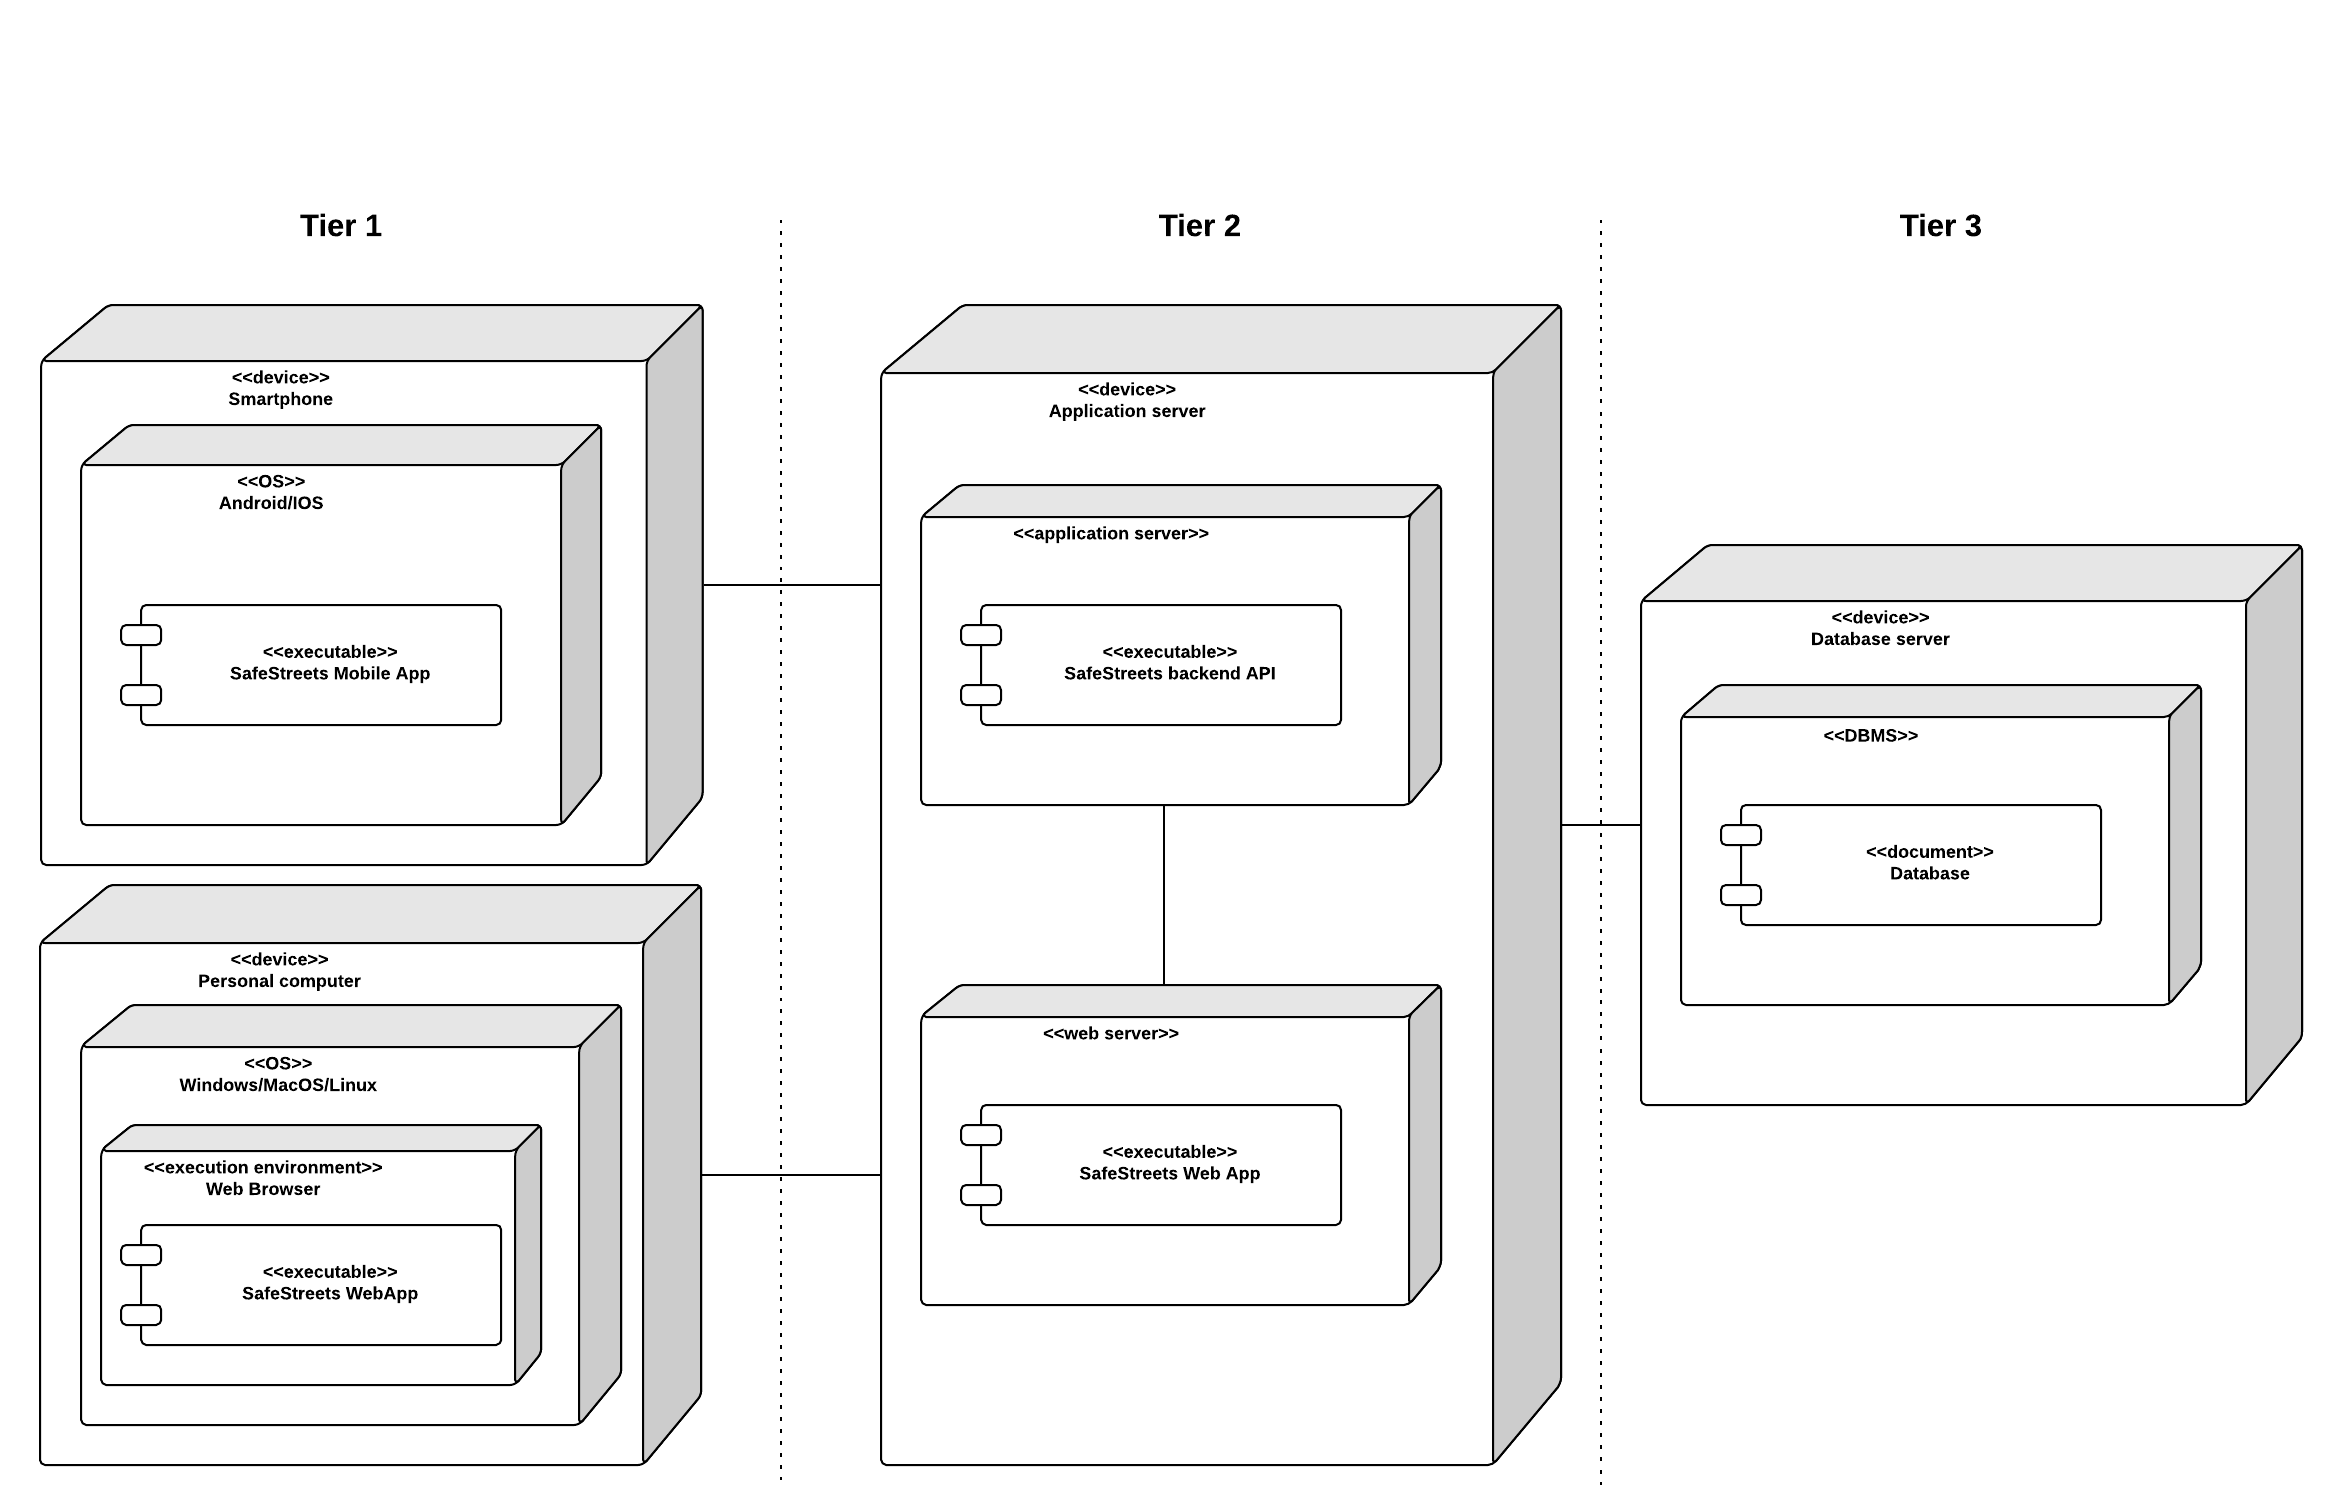
\includegraphics[width=1\textwidth]{Deployment_Diagram}
  \caption{Deployment diagram}
  \label{fig:deployment_diag}
\end{figure}

The diagram represents the architectural pattern chosen for the deployment of the SafeStreets service. It's a three-tiers architecture that has been conceived in order to provide a fast and lightweight client for both the users and the authorities. 
It is also important to note that the previous diagram is focused only on those components that will have to be effectively developed,that's why, for example, the plate recognitions services are not displayed in the diagram, as they already exists.
Here is a short explanation of what each tier does:
\begin{itemize}
  \item \textbf{Tier 1}: The first tier is the presentation tier of the architecture. The main function of this layer is to host  the application of the users and the Web app of the authorities. It is worth noting that there's little or nothing business logic present in this layer apart from those that are strictly required for the correct functioning of the applications; the mobile application and the Web App are only presentation client that will have to interact with the second tier in order to get/elaborate information. As for the deployment aspect: the mobile application must be developed in order to cover most of the devices, so it must be runnable at least on Android and IOS (to reduce the development time one could also think to use a cross-platform development framework) while the Web app must be compatible with the most modern web browser such as: Edge, Chrome, Firefox and Safari. As stated before, the applications in this tier are just thin clients so they need to interact with the application server in order to get information. The Mobile application asks the information directly to the application server via the backend API while the Web app communicate with the web server that will eventually ask to the application server for data. All the communications are performed with RESTful calls over a secure connection;
  \item \textbf{Tier 2}: The second tier of the architecture is called the logic layer. It is the layer in which all the business logic is located; all the functionalities and the elaborations are computed here. The implementation is achieved via a server that runs two subservices separately: the Application server and the Web server. The Application server hosts the core of the system that is to say the SafeStreets Backend API, this is the piece of software that will handle all of the requests and the offered services. Instead the Web server hosts the content for the web app. In case some pages need to be created with some data, the Web server can communicate with the backend API in order to retrieve the information needed;
  \item \textbf{Tier 3}: The final layer is the Data tier. It handles the data access with the remote databases. The choice to move this into a separate tier is due to the fact that with this approach data is independent from the business logic.
\end{itemize}

  \section{Runtime view}
  \subsection{Send a report}

This sequence diagram represents the process of the basic functionality of the app, that is to say the send report function. As soon as the user taps on the new report icon the app opens the camera interface so that the user can take the picture of the violation. Once the picture has been taken the app automatically gather from the phone the required data that need to be associated with the report, such as: GPS coordinates, date and time. Then a page that contains such data and a preview of the picture is shown to the user. In order to send a valid report he must also choose, from a list of violation category, the one that best suits the event; ultimately he can choose to modify the information as he wants (i.e. retake picture, change address, etc ...). Once the report is complete the application submits the report to the URIManager that will forward the request to the NewReportHandler component. This component will send to the PlateRecognitionService component the image in order to retrieve the plate number associated. Once the plate number is returned to the NewReportHandler the complete report is sent to the QueryManager that will perform an insert query on the database. After the insertion the latter will send the query result, in this case just a status message (i.e. correct saving), to the AggregationManager that will just forward the notification to the SendMobileNotificationManger. The SendMobileNotificationManger finally sends a push notification to the mobile app containing a message about the correct .
 

  \section{Component interfaces}
  \begin{figure}[H]
    \centering
    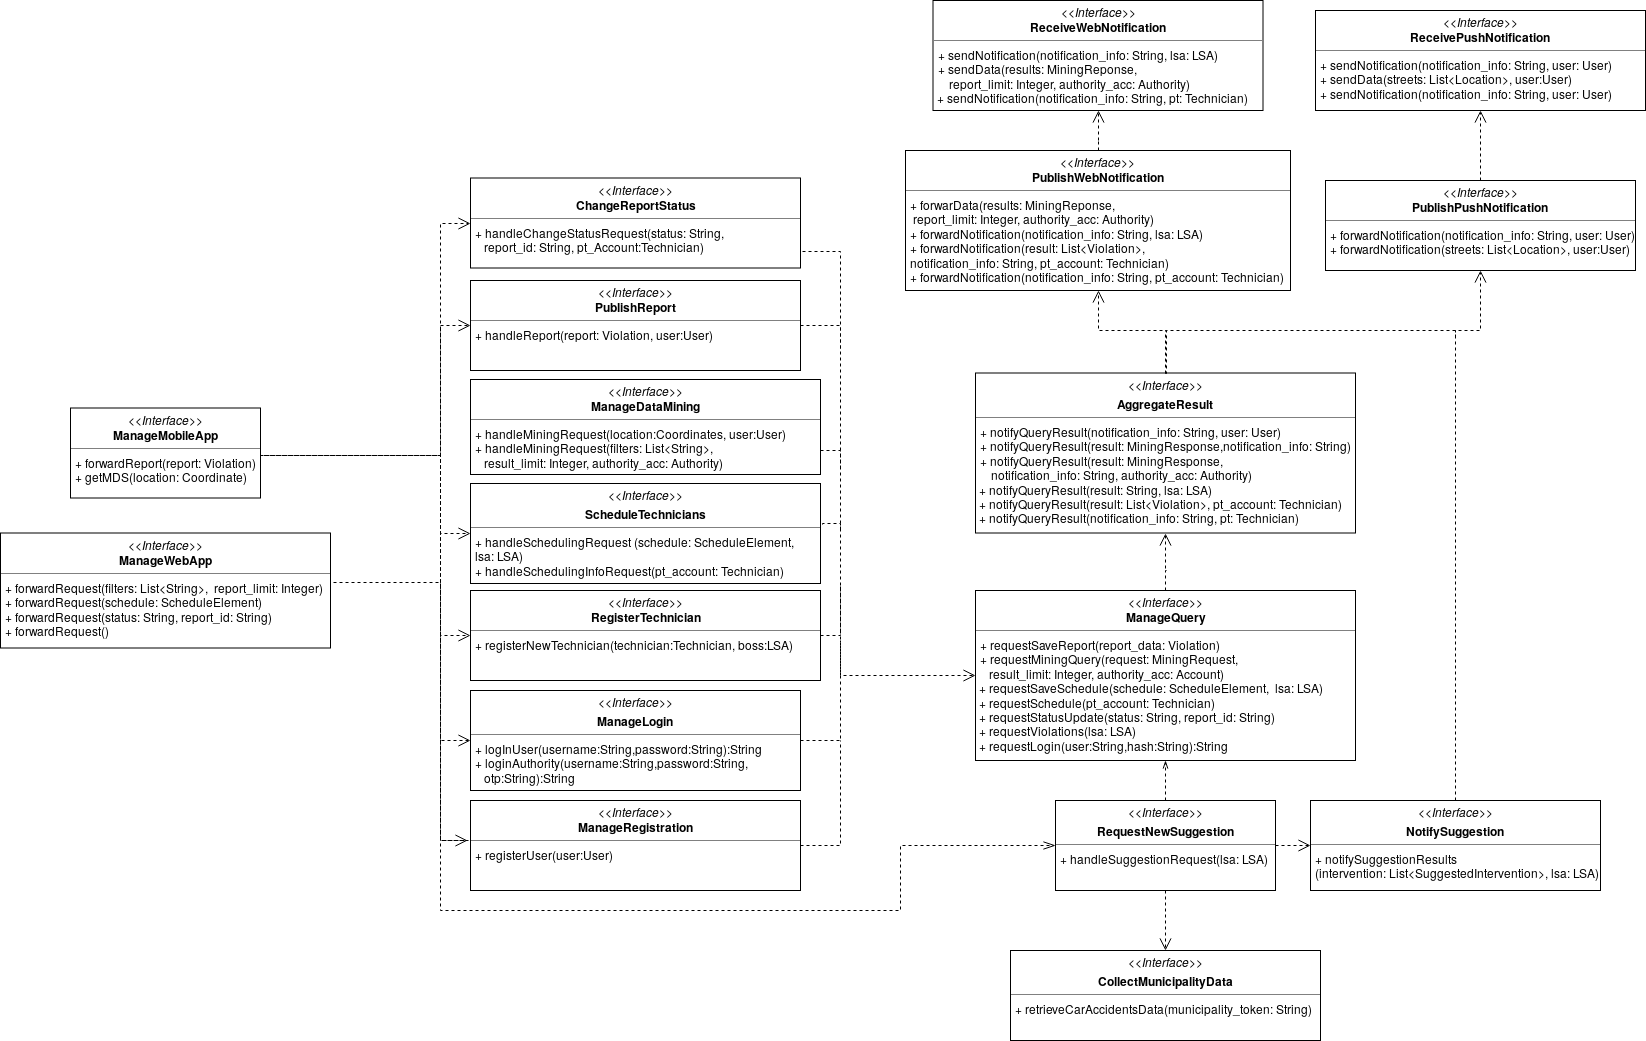
\includegraphics[width=1.1\textwidth]{UML_diagrams/interface_diagram_safestreets}
    \caption{Interface diagram}
    \label{fig:interface_diagram}
\end{figure}
In the figure \ref{fig:interface_diagram} the component interfaces belonging to the application server are represented with respect to what was shown in the Component diagram. The arrows represent dependency relations and depict the dependency tree of the application backend interfaces. 
The functions represented in the interface diagram have the following properties:
\begin{itemize}
    \item The signature of this functions are built only for conceptual showing purposes and they might differ in the final implementation;
    \item The main part of this diagram's functions have been pictured for guaranteeing a correct correspondency with the sequence diagrams of the previous paragraph, therefore some functions are submitted to the overloading technique;
    \item The interfaces are offered by the application backend component to one another or to other SafeStreets system components (mobile application and web application).
\end{itemize} 
In order to better understand how the interfaces work and how they are correlated, the following list of clarifications (assumptions) have been considered:
\begin{itemize}
    \item The frontend interfaces have been generically represented by the ReceivePushNotification and ReceiveWebNotification interfaces for dependency purposes. For the sake of simplicity, they have not been analyzed in depth as it is not relevant for the system global functioning;
    \item The workflow of the operation of the SafeStreets system is the following:
        \begin{itemize}
            \item In order to perform any of the functionalities offered by the application backend, the external applications interacts to the ManageMobileApp and ManageWebApp by a RESTful API service;
            \item The functions of these two interfaces forward the requests to the interface of the component related to the called API, propagating also all the parameters embedded to the request (if correctly formalized);
            \item When one of its function is called, the interface of the target component takes in charge the request and let the component do its computation;
            \item Once computation is done, the ManageQuery interface is called in order to interact with the database;
            \item At this point, the component related to the ManageQuery interface execute all the necessary queries and directly forwards the results to the AggregateResult interface;
            \item In this component, the result of the computation is formalized and forwarded to the PublishWebNotification interface in case the request came from a web application (LSA or Technician accounts) or from a mobile application (User)\textsuperscript{[1]};
            \item The publishing interfaces collect the responses and forward them to the devices that performed the operation\textsuperscript{[2]};
            \item The ReceiveWebNotification and ReceivePushNotification API interfaces receive asynchronously the responses and let the local applications handle them.
        \end{itemize}
    It is paramount to underline that the workflow of operations cannot be traversed in the opposite way. For this reason, all interface functions does not have a return type;
    \item The calls of the interfaces functions are performed synchronously: as explained at the previous point, the system operations flow only one way and the output of the previous ones is piped as input to the next one. Without a synchronous function calling system, the piping could not be implemented;
    \item The ManageQuery interface's functions don't have a queryType parameter because it can be inferred from the parameters of the functions: the requestMiningQuery function can be univocally inferred as a SELECT request, the requestSaveSchedule can be univocally inferred as an INSERT and so on;
    \item The ManageQuery interface is the only interface that leads to the QueryManager component. Therefore, all of the previous interfaces depend on it for query executions;
    \item The LoginManager's functions are the only ones that return a value (String): this is due to the authentication token, which has to be backpropagated to the URIManager component in order to perform its functions.
\end{itemize}
\textbf{\textsuperscript{[1]}}: all of the functions of the interfaces that requires a response have the submitter's account as a parameter: this is both necessary for the specific computation of the offered functions and for mapping the response to the submitter. If in some cases the account is not explicitly specified, it is because it can be retrieved by other parameters (e.g. requestSaveReport: the submitter is the violation.user).\newline
\textbf{\textsuperscript{[2]}}: the SafeStreets system handles a table with <Account, Address> tuples, which allows the Notification Service components to forward the results of computation.
\begin{figure}[H]
    \centering
    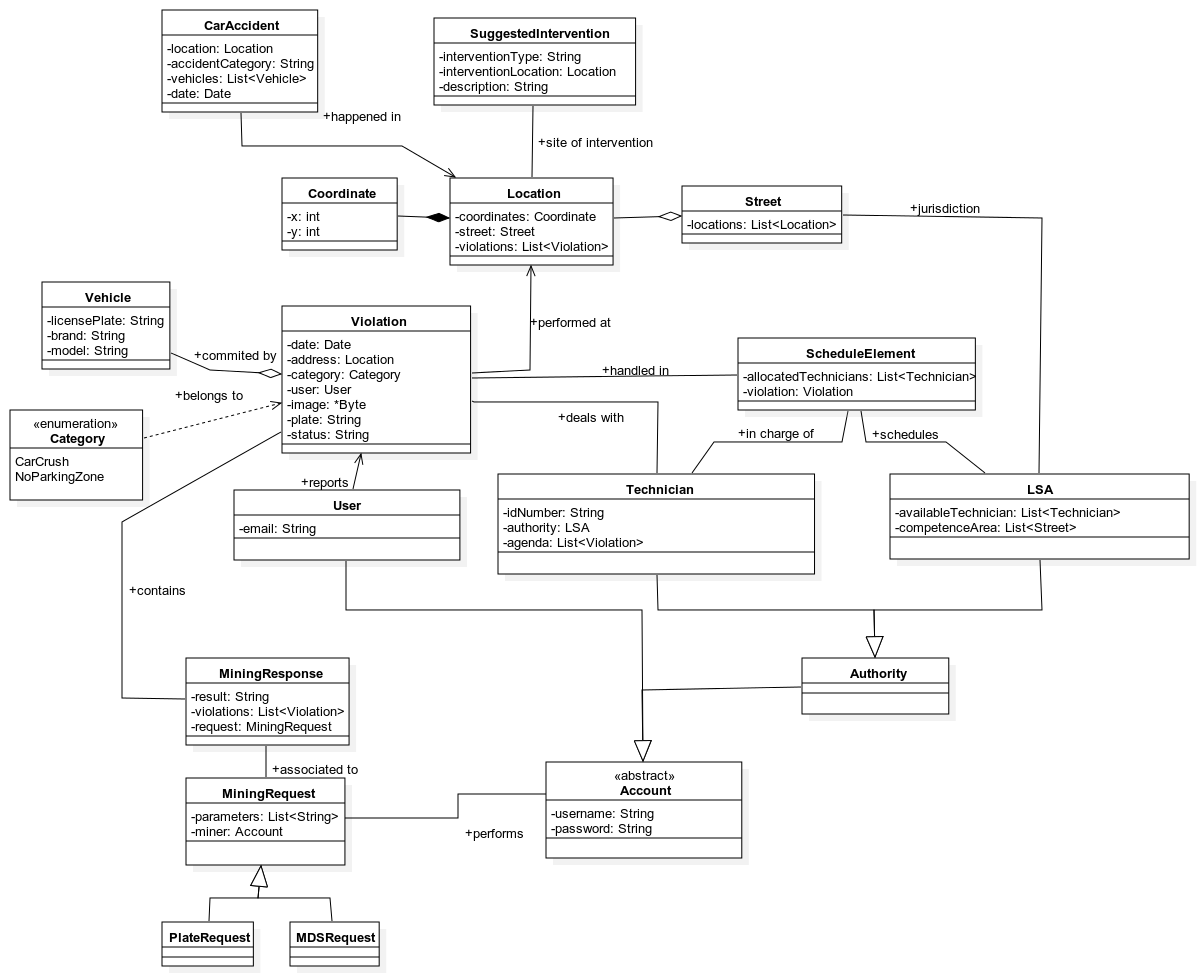
\includegraphics[width=1.1\textwidth]{UML_diagrams/class_diagram_safestreets}
    \caption{Class diagram}
    \label{fig:class_diagram}
\end{figure}
In figure \ref{fig:class_diagram}, the SafeStreets class diagram is represented. This version of the class diagram is similar to the one present in the RASD document, a part from:
\begin{itemize}
    \item The Mining request generalization, in order to add a new useful and extendible design pattern;
    \item The ScheduleElement class, which represents the n-n relation between Technicians and Violations: instead of representing this multiple relation in a singleton class which associate Technicians and Violations, the ScheduleElement objects represent tuples that links a single violation to many Technicians ($\le 5$ as stated in the RASD document). In this way, the system allows LSAs to schedule many Technicians to a specific violation as pictured in the web application mockups. The opposite operation (Technician to many violation) is not allowed up to this version of the system;
    \item The CarAccident class, which represent the aggregation of a single datum collected from the Municipality information system;
    \item The authority generalization of the classes LSA and Technician, in order to identify those classes of accounts which belongs to authorities, therefore they can perform a series of action which are forbidden to Users. 
\end{itemize}

  \section{Selected architectural styles and patterns}
  \subsection{RESTful	API architecture}
A RESTful API is based on representational state transfer (REST) technology, an architectural style and approach to communications often used in web services development.
A RESTful API breaks down a transaction to create a series of small modules. Each module addresses a particular underlying part of the transaction. This modularity provides developers with a lot of flexibility. Every specific module of the REST API can be invoked remotely by an URI which uniquely identifies that service. Once an API has been casted, a certain function is executed on the RESTful API server: the result of this computation is then sent back to the invoking client by a callback function that it offers.
As far as the SafeStreets system is concerned, both the web and the mobile application make use of RESTful APIs offered by the application backend system: 
\begin{itemize}
    \item the mobile application directly interacts with the APIs through their URIs;
    \item the web application retrieves data and performs operations that require the application backend system through API invokation through a \textbf{Promise-Deferred} asynchronous calling system.
\end{itemize}
Also, the mobile application make use of the Google Maps API for the mapping service.\newline
At the same time, the application backend system make use of the RESTful APIs offered by the Municipality information system and the Image recognition service.
Therefore, a certain information system can be both offering and using RESTful APIs for its purposes.
\subsection{MVC design pattern}
As deeply explained in the overview paragraph of this section, the MVC design pattern is the core of the functioning of the SafeStreets system.
In order to provide a detailed explanation of how this popular design pattern works, here it is a detailed description from the  Wikipedia website:
\begin{itemize}
    \item \textbf{Model}:\textit{" The central component of the pattern. It is the application's dynamic data structure, independent of the user interface. It directly manages the data, logic and rules of the application."}
    \item \textbf{View}: \textit{"Any representation of information such as a chart, diagram or table. Multiple views of the same information are possible, such as a bar chart for management and a tabular view for accountants."}
    \item \textbf{Controller}:\textit{"Accepts input and converts it to commands for the model or view.
    In addition to dividing the application into these components, the model–view–controller design defines the interactions between them.
    The model is responsible for managing the data of the application. It receives user input from the controller.
    The view means presentation of the model in a particular format.
    The controller responds to the user input and performs interactions on the data model objects. The controller receives the input, optionally validates it and then passes the input to the model.
    As with other software patterns, MVC expresses the "core of the solution" to a problem while allowing it to be adapted for each system."}
\end{itemize}
The main advantages that the MVC design pattern provides are:
\begin{itemize}
    \item Simultaneous development – Multiple developers can work simultaneously on the model, controller and views;
    \item High cohesion – MVC enables logical grouping of related actions on a controller together. The views for a specific model are also grouped together;
    \item Loose coupling – The very nature of the MVC framework is such that there is low coupling among models, views or controllers;
    \item Ease of modification – Because of the separation of responsibilities, future development or modification is easier;
    \item Multiple views for a model – Models can have multiple views.
\end{itemize}
In the SafeStreets system, the model is represented by the Cloud DBMS and the DataQueryService subsystem of the backend application and the MunicipalityDataHandler of the SuggestedInterventionService;
the view is represented by the web and mobile application; the controller is represented by all the application backend subsystem except from the DataQueryService and the MunicipalityDataHandler of the SuggestedInterventionService.
\subsection{Three-tier architecture}
Three-tier architecture is a client-server software architecture pattern in which the user interface (presentation), functional process logic ("business rules"), computer data storage and data access are developed and maintained as independent modules, most often on separate platforms. The Wikipedia website states that in the three-tier architecture it is possible to evidence:
\begin{itemize}
    \item \textbf{Presentation tier}: 
    \textit{"This is the topmost level of the application. The presentation tier displays information. It communicates with other tiers by which it puts out the results to the browser/client tier and all other tiers in the network. In simple terms, it is a layer which users can access directly (such as a web page, or a mobile application)."}
    \item \textbf{Application tier}: \textit{
    "The logical tier is pulled out from the presentation tier and, as its own layer, it controls an application’s functionality by performing detailed processing."}
    \item \textbf{Data tier}: \textit{
        "The data tier includes the data persistence mechanisms (database servers, file shares, etc.) and the data access layer that encapsulates the persistence mechanisms and exposes the data. The data access layer should provide an API to the application tier that exposes methods of managing the stored data without exposing or creating dependencies on the data storage mechanisms. Avoiding dependencies on the storage mechanisms allows for updates or changes without the application tier clients being affected by or even aware of the change. As with the separation of any tier, there are costs for implementation and often costs to performance in exchange for improved scalability and maintainability."}
\end{itemize}
Although the three-tier architecture may seem very similar to the MVC design pattern, they present a crucial difference: in the three-tier architecture the client tier is forbidden to communicate with the data tier (as it is implemented in the SafeStreets system) while the communication in the MVC pattern is triangular. As far as the SafeStreets sytem is concerned, only the application tier is responsible for the interactions between different layers.
  \section{Other design decisions}
  \subsection{Lightweight thin client}
The client software is narrowly purposed and lightweight: only the host server or server farm needs to be secured,rather than securing software installed on every endpoint device (although thin clients may still require basic security and strong authentication to prevent unauthorized access). One of the combined benefits of using cloud architecture with thin client desktops is that critical IT assets are centralized for better utilization of resources. Unused memory, bussing lanes, and processor cores within an individual user session, for example, can be leveraged for other active user sessions.
\newline
The simplicity of thin client hardware and software results in a very low total cost of ownership, but some of these initial savings can be offset by the need for a more robust cloud infrastructure required on the server side. Therefore, the SafeStreets mobile application can be run on any device (even cheap ones) as the computational power required is extremely low.
\newline
Mobile devices and web browser are responsible only for showing the results of the computation of the backend system: this functiong allows to speed up the execution of the system functions that are performed on a powerful hardware on the server side.
\subsection{Relational database}
Relational databases are the most used technique of data storaging. A relational database has at least to guarantee the following aspects:
\begin{itemize}
    \item Present the data to the user as relations (a presentation in tabular form, i.e. as a collection of tables with each table consisting of a set of rows and columns);
    \item Provide relational operators to manipulate the data in tabular form.
\end{itemize}
In order to build a formally correct relational database, it is necessary to create a \textbf{Relation model} of the data that the database is going to contain. The relational model organizes data into one or more tables (or "relations") of columns and rows, with a unique key identifying each row. Rows are also called records or tuples.Columns are also called attributes. Generally, each table/relation represents one "entity type" (such as user or violation). The rows represent instances of that type of entity  and the columns representing values attributed to that instance (such as username or date). 
\newline Moreover, tables are connected through relations, which are a logical connection, established on the basis of interaction among these tables. 
\newline In order to interact with a relational database, it is necessary to use a RDBMS, such as PostgreSQL or MySQL and so forth.
\newline The main advantages of using a relational database are:
\begin{itemize}
    \item \textbf{Accuracy}: Data is stored just once, eliminating data deduplication;
    \item \textbf{Flexibility}: Complex queries are easy for users to carry out;
    \item \textbf{Collaboration}: Multiple users can access the same database;
    \item \textbf{Trust}: Relational database models are mature and well-understood;
    \item \textbf{Security}: Data in tables within a RDBMS can be limited to allow access by only particular users.
\end{itemize}
In the SafeStreets system, relational databases are very useful as: 
\begin{itemize}
    \item data is structured in a fixed way, therefore NoSQL databases are not very useful;
    \item many users and authorities accounts have to perform frequent queries to the DB;
    \item the hierarchical structure of the RDBMS allow SafeStreets to perform some of the privileges controls directly on the inside the RDBMS.
\end{itemize}
\subsection{Cloud database}
A cloud database is a database that typically runs on a cloud computing platform, and access to the database is provided as-a-service.
Database services take care of scalability and high availability of the database. Database services make the underlying software-stack transparent to the user.
The design and development of typical systems utilize data management and relational databases as their key building blocks. Advanced queries expressed in SQL work well with the strict relationships that are imposed on information by relational databases. However, relational database technology was not initially designed or developed for use over distributed systems. This issue has been addressed with the addition of clustering enhancements to the relational databases, although some basic tasks require complex and expensive protocols, such as with data synchronization.
\newline The main advantages of adopting a cloud DBMS are:
\begin{itemize}
    \item Scalability: scaling along any dimension generally requires adding or subtracting nodes from a cluster to change the storage capacity, I/O operations per second, or total compute available to bring to bear upon queries. That operation, of course, requires redistributing copies of the data and sending it between nodes. Although this was once one of the hardest problems in building scalable, distributed databases, the new breed of cloud-native databases can take care of these issues efficiently;
    \item Reduced Administrative Burden: a cloud-hosted, mostly self-managed database doesn’t eliminate a database administrator, but it can eliminate unnecessary features that typically consume much of a DBA’s time and efforts. That allows a DBA to focus his or her time on more important issues;
    \item Improved Security: by running databases on in-house servers, it’s SafeStreets responsibility to think about security. It is necessary to ensure that databases have an updated kernel and other critical software, and it is necessary to keep up with the newest digital threats. By delegating all these operations to the cloud DBMS company, a lot of work is saved.
\end{itemize}
All of this advantages relieves an heavy burden from the budget of the project, as the expenses of a Cloud DBMS service is much lower than affording a local DBMS.
  
  \chapter{User interface design}
  Since the mockups of the mobile application and the web application were already added in the RASD document, here they are presented two flowchart-like diagrams that represent the user navigation flow in both applications. It is implicit that if the users click the back button the apps return to the previous page, as it happens in all common applications.

\vfill

\begin{figure}[H]
  \centering
  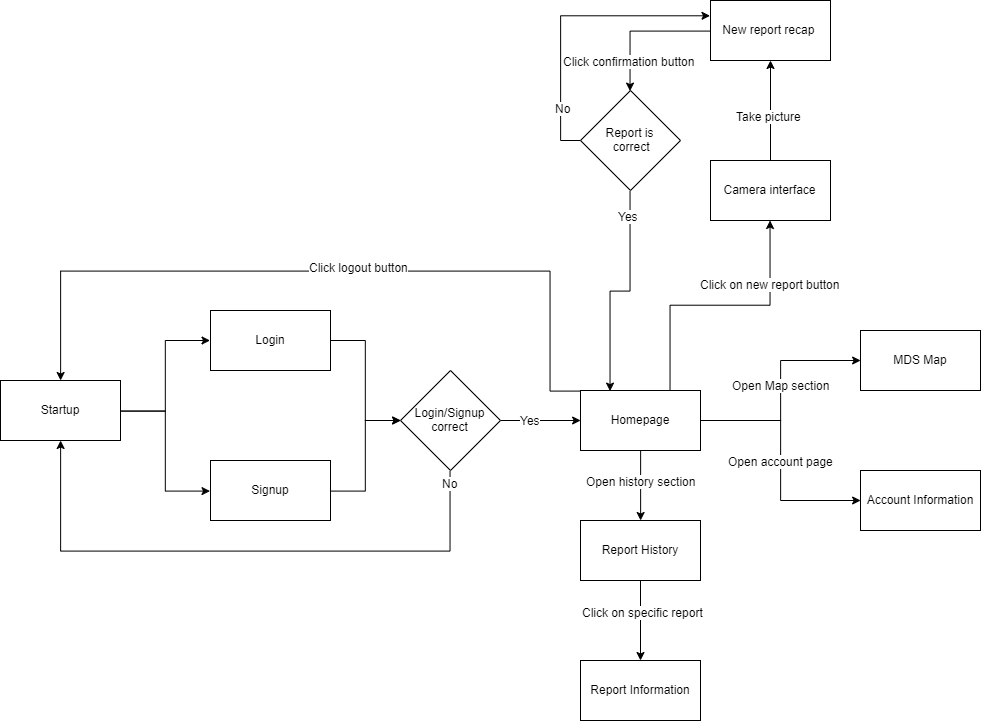
\includegraphics[width=1\textwidth]{Images/UI_Mobile_App.png}
  \caption{UI diagram of the mobile application}
  \label{fig:ui_mobile_app}
\end{figure}

\vfill
\newpage
\null
\vfill

\begin{figure}[H]
  \centering
  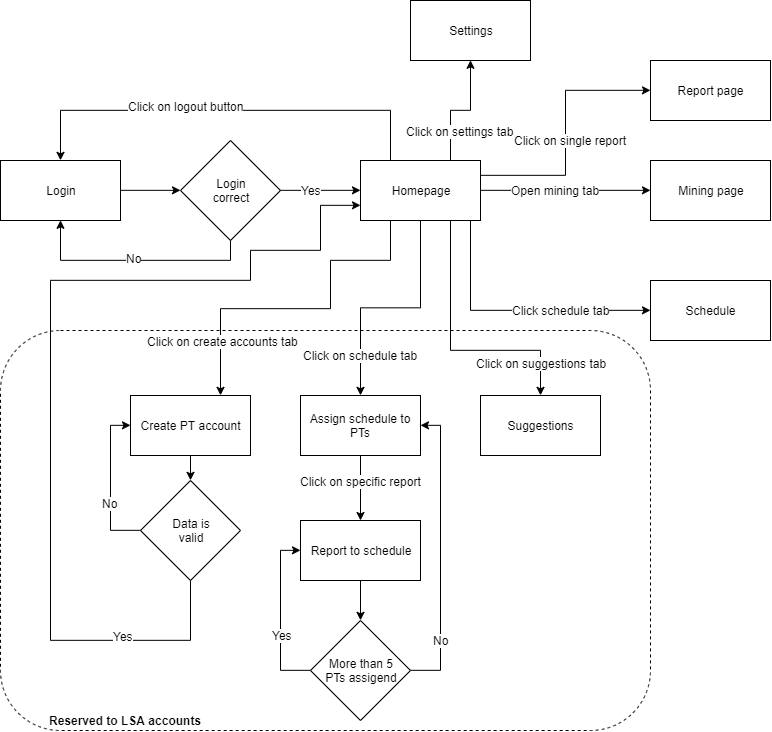
\includegraphics[width=1\textwidth]{Images/UI_Web_App.png}
  \caption{UI diagram of the web application}
  \label{fig:ui_web_app}
\end{figure}


\vfill
\newpage

  
  \chapter{Requirements traceability}
  In this chapter we exhibit the mapping between the requirements stated in the RASD document and the design elements that have been introduced in order to address them. The stated components can sometimes address the requirements independently but some other times they rely on the actions of other components, such behaviour it is however illustrated in the description if needed. 

\begin{itemize} 
    \item {[R1]}: The mobile application must be able to gather all the required data such as: location, date and time from the user's device;
    \item[] {[R2]}: The mobile application has to allow the user to choose between different categories of violations;
    \item[] {[R3]}: The mobile application has to allow the user to optionally add information about the event and the car plate number;
    \item[] {[R4]}: The mobile application has to allow the user to retake the picture if desired;
    \begin{itemize}
      \item \textbf{UserMobileApp}: this component, that represents the mobile application, is responsible to handle all this kind of user experience requirements.
    \end{itemize}
    \item {[R5]}: The mobile application must be able to interact with the backend system to send/retrieve information.
    \begin{itemize}
      \item \textbf{UserMobileApp}: this component, in order to connect to the backend, handles the connection with the URIManager directly.
    \end{itemize}      
    \item {[R6]}: The backend system must be able to send the violation image to the plate recognition service in order to retrieve the car plate number from the image;
    \begin{itemize}
      \item \textbf{NewReportHandler}: this component, after some checks on the correctness of the violation report, sends the image to the PlateRecognitionService.
    \end{itemize}  
    \item {[R7]}: Once the car plate number has been retrieved the system must save the report information in the database;
    \begin{itemize}
      \item \textbf{QueryManager}: under the request submitted by the NewReportHandler, the QueryManager will save the plate number, along with the other information, in the database. 
    \end{itemize} 
    \item {[R8]}: The backend system must retrieve the latest reports submitted by the user from the database. Once the data is gathered, the backend system must send it to the mobile application that will display them; 
    \item[] {[R9]}: The user must be able to consult the status associated with each report;
    \begin{itemize}
      \item \textbf{FilteringManager}: the FilteringManager manages also the requests regarding the history of reports of a specific user. This component will ask to the QueryManager to retrieve such data, after the data are obtained they are forwarded back to the mobile application through the SendMobileNotificationManager.
    \end{itemize}
    \item {[R10]}: The application has to allow the user to insert an address near which to search the MDS. If no address is provided the application will instead search the MDS near the current position of the user (collected from the GPS);
    \begin{itemize}
      \item \textbf{UserMobileApp}: this behaviour is handled by the mobile application, if an address is provided it will be used, instead of the GPS coordinates, to formulate the MDS request.  
    \end{itemize} 
    \item {[R11]}: The backend system must calculate the MDS close to the given location;
    \begin{itemize}
      \item \textbf{AggregationManager}: this component calculates the MDS immediately after the QueryManager provides to it the necessary data; 
    \end{itemize} 
    \item {[R12]}: The mobile application must enlighten on the map the MDS;
    \begin{itemize}
      \item \textbf{UserMobileApp}: the UserMobileApp component asks to the map service to display the map along with the MDS highlighted.
    \end{itemize} 
    \item {[R13]}: The Web application must be able to interact with the backend system to send/retrieve information;
    \begin{itemize}
      \item \textbf{AuthorityWebServer}: through the requests forwarded by the AuthorityWebServer to the URIManager the web application is effectively interacting with the backend system.
    \end{itemize}     
    \item {[R14]}: The Web application must provide a special interface for the LSA in order to perform special task reserved for his role;
    \begin{itemize}
      \item \textbf{AuthorityWebApp}: this component represents the web app itself.
    \end{itemize}  
    \item {[R15]}: The Web application must allow the LSA to securely create account reserved for PT;  
    \item[] {[R16]}: The Web application must allow the LSA to associate the PT's badge number with his related account;
    \item[] {[R17]}: The system automatically generates a temporary password associated to the new account. Upon the first login, the application asks the PT to change the password;
    \item[] {[R18]}: The system correctly registers the new accounts and allows access to the Web application to the PT registered;
    \begin{itemize}
      \item \textbf{TechnicianRegistrationManager}: this component is entirely dedicated to handle all the necessary procedures related to the creation of a new PT account. Clearly in order to save the newly created account this component will have to interact with the QueryManager.
    \end{itemize} 
    \item {[R19]}: The Web application allows the visualization of reports to both the LSA and the PTs via a dedicated section;
    \begin{itemize}
      \item \textbf{FilteringManager}: as soon as the authority opens the web application a request is sent to this component that will gather the necessary query parameter and then perform another request to the QueryManager to retrieve such data.
    \end{itemize}    
    \item {[R20]}: The Web application allows the LSA to schedule reports to PT by associating their account to the report;
    \item[] {[R21]}: The Web application allows PTs to visualize their scheduled reports;
    \begin{itemize}
      \item \textbf{SchedulingManager}: this component handles the process of associating PTs to reports done by the LSA to create the schedule. It also handles the request of consulting the personal PT schedule by performing a query for such schedule on the QueryManager.
    \end{itemize}
    \item {[R22]}: The Web application allows both the LSA and the PTs to change the status of reports (i.e. from "PENDING" to "SOLVED");
    \begin{itemize}
      \item \textbf{ViolationStatusManager}: this component has been designed to address this purpose.
    \end{itemize}
    \item {[R23]}: The Web application provides a section that can be used by both LSA and PTs to mine the data.
    \item[] {[R24]}: The system must be able to collect the filter criteria inserted by the authorities and then compose a query that will be executed to retrieve the matching data;
    \item[] {[R25]}: The Web application provides a section that can be used by both LSA and PTs to visualize statistics/metrics about the data;
    \item[] {[R26]}: The system must offer some functionalities to calculate the most useful statistics/metrics related to the data;
    \begin{itemize}
      \item \textbf{AuthorityWebApp}: some sections of this web application are developed in order to create an interface that allows authority to mine data and get useful metrics;
      \item \textbf{FilteringManager}: this component, based on the filters inserted by the authority, gathers a list of query parameters that will we passed over to QueryManager in order to retrieve the desired data. It also provides the functionalities needed to calculate the most useful metrics and statistics.
    \end{itemize}    
    \item {[R27]}: The Web application provides a section from which the authorities can ask for suggestions;
    \begin{itemize}
      \item \textbf{AuthorityWebApp}: a dedicated section in the web application serves this purpose.
    \end{itemize}     
    \item {[R28]}: The backend system must be able to communicate and retrieve data from the municipality service at any given time;
    \begin{itemize}
      \item \textbf{MunicipalityDataHandler}: this component performs the request to the MunicipalityDataSharing system in order to retrieve the car accidents data.
    \end{itemize}
    \item {[R29]}: The system has to merge and find correlations between the violations and the car accidents;
    \item[] {[R30]}: The system has to identify potentially unsafe areas and then estimate possible interventions based on the correlations that have been found;
    \begin{itemize}
      \item \textbf{SuggestionGenerationManager}: this component performs the sequence of operations required to produce the suggested intervention; such as requesting the data to the MunicipalityDataHandler, crossing the data and calculating the suggestions.
    \end{itemize}
    \item {[R31]}: Once the computation is over the Web application must display the suggested interventions on the interface along with the location;
    \begin{itemize}
      \item \textbf{SuggestionNotifier}: once the suggestions are produced they are sent over to the this component that will forward them back to the web application through the SendNotificationWebManager.
    \end{itemize}
\end{itemize}

  
  \chapter{Implementation, integration and test plan}
  The SafeStreets system is divided into three main application:
\begin{itemize}
    \item The Mobile application;
    \item The Web application;
    \item The backend application.
\end{itemize}
Every application enlisted above will be developed, tested and integrated following a bottom-up strategy. Firstly, the backend application will be developed as it creates a dependency to the mobile and the web application: without a functioning backend, it would be necessary to create a series of drivers in order to test the functionalities of the frontend applications. Once the backend application will be implemented and tested with respect to the majority of its components (the most relevant ones), it will be possible to continue with the development and testing of the mobile and web application. In the end, the whole system will be integrated and tested.
For the sake of simplicity, this document will cope with the the implementation, testing and integration of the backend application.
\subsection{Backend application implementation}
As previously explained in the component diagram, the backend application is divided into several subsystems, which wrap up all the components that perform similar tasks. Moreover, every subsystem is composed by a set of components which represent the atomic elements of the system.
The implementation process will start from those components that create a lot of dependencies to other components (for example the QueryManager) and will continue with the remaining ones. After having unit-tested every function implemented, each component will be integrated and tested as a whole. 
The main rationale behind the style of the development and testing that have been selected is functionality-wise rather than component-wise: instead of building a whole component as once, only the functions which are needed to perform a specific functionality are assembled. Moreover, an incremental integration and testing of such components will be performed until the functionality will be considered ready to be deployed.

In order to proceed with the implementation of the SafeStreets system functionalities, the following table has been created expressing for each functionality the difficulty of implementation and testing and the level of importance to customers.
\begin{table}[H]
    \centering
    \begin{tabularx}{\textwidth}{ |l|c|c| }
        \hline
        Functionality & Level of importance & Difficulty \\
        \hline
        Register and LogIn & low & low \\								
        \hline
        View history of reports & medium & low \\
        \hline
        Create a new report & high	& medium \\
        \hline								
        Schedule police technicians & medium & medium \\									
        \hline
        Watch own schedule & medium & low \\									
        \hline
        Register a new technician & medium & medium \\
        Perform information mining & high & high \\									
        \hline
        Change report status & high & low \\									
        \hline
        Generate suggested intervention & medium & high \\									
        \hline
    \end{tabularx}
  \end{table}
The levels of importance and difficulty have been determined in an arbitrary way, based on the experience.
In order to explain more in detailes the order of implementation and which components have to be implemented, here it is a list of precedence that will have to be followed while implementing and testing:
\begin{itemize}
    \item \textbf{Perform information mining}: firstly it is necessary to develop the QueryManager, which performs the interactions with the ViolationDB and the AggregationManager as next. After this, it will be possible to proceed with the FilteringManager as it requires the interaction with the QueryManager. As soon as the previous components have been integrated, it will be possible to develop and test the
     SendNotificationWebManager and the SendNotificationMobileManager. The implementation of the latters can be performed asynchronously as they do not create any dependencies one another; 
    \item \textbf{Create a new report}: the first component to be developed is the NewReportHandler: it depends on the QueryManager which will need to be integrated with the functionalities required and the external service of image recognition for the license plates. As this latter component is external, it will be treated as well functioning and tested. The same process of integration of functions to actuate the "Create new Report" functionality will continue with the rest of the flow described at the previous point: QueryManager, AggregationManager,SendNotificationWebManager and (in parallel) SendNotificationMobileManager;
    \item \textbf{Change report status}: this functionality requires the development and testing of the ViolationStatusManager. All the (same) chain of dependencies will be updated and integrated with the functions needed for performing the "Change report status";
    \item \textbf{Generate suggested intervention}: this functionality requires the development of the whole SuggestedIntervention Service subsystem: firstly, the development process should start from the MunicipalityDataHandler, which is in charge to interact with the Municipality information system (black box). Once this component has been developed, it will be time to proceed with the SuggetionGenerationManager that will interact with the MunicipalityDataHandler and the QueryManager to perform its computation. For this reason, the the QueryManager will be updated as necessary. At this moment, the SuggestionNotifier will be implemented and the SendNotificationMobileManager and SendNotificationWebManager will be updated aswell. The whole SuggestedIntervention Service subsystem should be fully implemented, tested and integrated at this point;
    \item \textbf{Schedule police technicians}: in order to perform this functionality, the SchedulingManager component should be developed as first, together with the update of the whole flow from the QueryManager to the SendNotificationWebManager and SendNotificationMobileManager. Now the QueryManager should be able to interact with the PersonnelDB;
    \item \textbf{Register a new technician}: this operation requires the development of the TechnicianRegistrationManager and the update of the whole flow from the QueryManager to the SendNotificationMobileManager and SendNotificationWebManager. Now the QueryManager should be able to interact with the AuthenticationDB, in order to store credentials of new technicians;
    \item \textbf{View history of reports}: this functionality requires the update of the FilteringManager and the QueryManager.  At this moment of the development, the Violation Service subsystem should be completely implemented, tested and integrated;
    \item \textbf{Watch own schedule}: this functionality requires the update of the SchedulingManager and the QueryManager. At this point of the development, the whole Personnel Service subsystem should be implemented, tested and integrated;
    \item \textbf{Register and LogIn}: this functionality requires the development, testing and integration of the whole Authentication service: the LogInManager and the RegistrationManager can be developed in the meantime, as they do not depend one another. The QueryManager will be updated. At this point, the Authentication Service subsystem should be completely implemented, tested and integrated. Also, it is possible to consider the Notification Service and Data Query Service subsystems as complete.
\end{itemize}
Lastly, the URIManager component is developed, tested and integrated with the rest of the system for enabling the RESTful API communication with the frontend and the mapping of such request.
The order of the list takes into account at first the level of importance to customers and then the level of difficulty for implementing and testing the specific functionality.


  \section{Verification and validation}
  The validation and verification phases should be actuated throughout the development process since its earliest phases: the later a certain bug/bad behaviour is detected, the higher the cost for solving it. Thus, each function should come together with its own unit test.\newline
Another set of test should be implemented when multiple functions are bound together to perform (part of) the functionality they address: this process allow the immediate detection of integration bugs which can result to be hard to detect when multiple functions are ensembled together (it could be very hard to detect in which exact point of the computation the bug is generated).
Once the first version of the SafeStreets system has been implemented and tested, some regression tests have to be developed in order to check the functioning of the system in the future releases.

  \section{Component integration}
  The backend component integration should procede as described in the chapter 5.0.1, therefore it is unnecessary to repeat it in this section.
Despite this, the component integration between the frontend, the backend and all the other external service requires a deeper explanation by the following diagrams.
\section{Frontend-Backend application}
Firstly, the AuthorityWebApp requires a server on which it is to be hosted. Therefore, it will be deployed on the AuthorityWebServer component.
Also, the frontend components has to be integrated with the URIManager in order to ask for RESTful APIs, as described in the figure \ref{fig:frontend_urimanager_i_diagram}.
\begin{figure}[H]
    \centering
    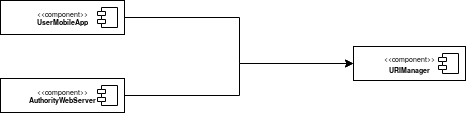
\includegraphics[width=.4\textwidth]{frontend_urimanager_i_diagram}
    \caption{Frontend-URIManager integration diagram}
    \label{fig:frontend_urimanager_i_diagram}
\end{figure}
On the other way, the Notification Service component has to be integrated with the respective frontend components, as described in fig. \ref{fig:notification_frontend_idiagram}
\begin{figure}[H]
    \centering
    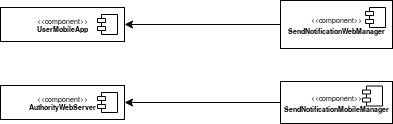
\includegraphics[width=.4\textwidth]{notification_frontend_idiagram}
    \caption{Notification-Frontend integration diagram}
    \label{fig:notification_frontend_idiagram}
\end{figure}
As far as the Cloud Database is concerned, the QueryManager has to be integrated with it as part of the data layer.
Finally, the external services have to be integrated with all the component that they require in order to perform their computation. The fig \ref{fig:external_services_idiagram} explains this matter in details.
\begin{figure}[H]
    \centering
    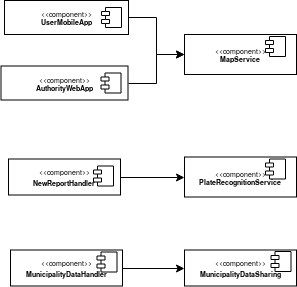
\includegraphics[width=.4\textwidth]{external_services_idiagram}
    \caption{External services integration diagram}
    \label{fig:external_services_idiagram}
\end{figure}
  
  \chapter{Effort Spent}
  \section{Luca Loria}
\begin{table}[H]
    \centering
    % \renewcommand{\arraystretch}{0.8}
    \begin{tabularx}{\textwidth}{ |l|c|X| }
        \hline
        Day & Hours & Topic \\
        \hline
        20/10/2019 & 1.5 & Text assumptions \\								
        \hline
        22/10/2019 & 1	& Domain assumptions \\
        \hline
        23/10/2019 & 2	& Design constraints \\
        \hline								
        24/10/2019 & 2	& Revision ch 1 and 2 \\									
        \hline
        26/10/2019 & 3 & Software system attributes \\									
        \hline
        28/10/2019 & 0.5 & Performance requirements \\									
        \hline
        29/10/2019 & 2	& External interface req \\									
        \hline
        30/10/2019 & 5 & Mockups creation \\									
        \hline
        31/10/2019 & 1.5 & Revision ch 3 \\									
        \hline
        01/11/2019 & 1 & Alloy signatures \\									
        \hline
        04/11/2019 & 1.5 & Alloy facts part 1 \\									
        \hline
        06/11/2019 & 3 & Alloy facts part 2 and world predicates \\						
        \hline
        07/11/2019 & 4 & Finish alloy, fix class diagram and start impaginating \\		
        \hline
        08/11/2019 & 3.5 & Reviewing requirements and sequence diagrams. Create references and Revision. Create alloy world section in RASD. Start impaginating correctly	\\
        \hline
        09/11/2019 & 2 & Shared phenomena matrix, frontpage and pagination fixes \\
        \hline							
    \end{tabularx}
  \end{table}

  \section{Nicolò Albergoni}
\begin{table}[H]
  \centering
  % \renewcommand{\arraystretch}{0.8}
  \begin{tabularx}{\textwidth}{ |l|c|X| }
      \hline
      Day & Hours & Topic \\
      \hline
      22/10/2019 & 2.5 & Purpose \\								
      \hline
      23/10/2019 & 3 & Scope, Current system \\
      \hline
      24/10/2019 & 1.75	& Goals, Overview\\
      \hline								
      26/10/2019 & 3	& Product perspective, Product function\\									
      \hline
      27/10/2019 & 3 & Product function, Revision ch 1 and 2 \\									
      \hline
      29/10/2019 & 2.5 & Scenarios \\									
      \hline
      30/10/2019 & 4 & Use cases \\									
      \hline
      31/10/2019 & 3 & Use cases, Revision ch 3 \\
      \hline
      01/11/2019 & 1 & Finish use cases \\									
      \hline
      02/11/2019 & 2.75 & Requirements \\									
      \hline
      05/11/2019 & 2.25 & Finish requirements \\									
      \hline
      06/11/2019 & 2.5 & Sequence diagrams \\									
      \hline
      07/11/2019 & 3.25 & Sequence diagrams \\						
      \hline
      08/11/2019 & 1.75 & Finish and reviewing of sequence diagrams \\
      \hline
      09/11/2019 & 2 & Use case diagrams, pagination fixes	\\
      \hline
      10/11/2019 & 2 & Traceability matrix, final revision	\\
      \hline        							
  \end{tabularx}
\end{table}


  \chapter{References}
  \begin{itemize}
    \item LateX Workshop extension for Visual Studio Code: \newline\href{https://github.com/James-Yu/LaTeX-Workshop/}{https://github.com/James-Yu/LaTeX-Workshop/}
    \item LateX compiler: \newline\href{https://www.latex-project.org/}{https://www.latex-project.org/}
    \item StarUML for UML diagrams:\newline\href{http://staruml.io/}{http://staruml.io/}
    \item DrawIO for some UML diagrams\newline\href{http://draw.io}{http://draw.io}
    \item MVC design pattern wikipedia: \newline\href{https://en.wikipedia.org/wiki/Model-view-controller}{https://en.wikipedia.org/wiki/Model-view-controller}
    \item Multitier architecture wikipedia: \newline\href{https://en.wikipedia.org/wiki/Multitier_architecture}{wikipedia}
    \item Relational database advantages: \newline\href{https://searchdatamanagement.techtarget.com/definition/relational-database}{https://searchdatamanagement.techtarget.com/definition/relational-database}
\end{itemize}
  \end{document}
  

  \loadspellchecklist[en][wordlist.txt]
  \setupspellchecking[state=start]
